\pagebreak

\huge Continuous Random Variables\\\normalsize~\\
A \underbar{~~~~~~~~~~~~~~~~~~~~~~~~~~~~~~~~~~~~~~~~~~~~~~~} has an interval or collection of intervals as its support\\
Ex:
\bi
\item $Y$=maximum daily temperature (interval $[-40^\circ F, 130^\circ F]$).
\item $Y$=lifetime (in years) of electronic equipment $0 <Y <\infty$
\item $Y$=weight loss (or gain) after a 6 month period $-\infty < Y < \infty$.
\ei

For Discrete RVs we had the probability distribution, $P(y)=P(Y=y)$.\\~\\
For Continuous RVs we can't assign probability to every $y$ in the support.  We now call the probability distribution by \\~\\

\bi
\item Probability a randomly chosen value will lie between any 2 given values is represented in terms of the area between the two values under the probability distribution.
\ei
\begin{center}
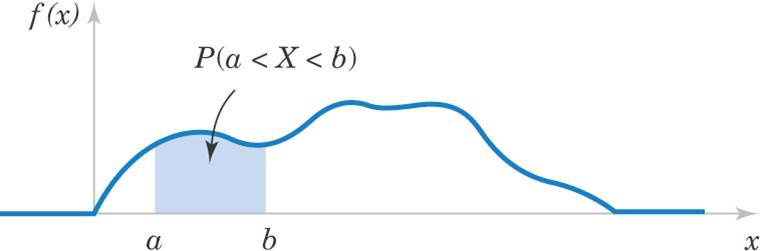
\includegraphics[width=3.5in, height=1in]{chapter4/pdf.jpg}\\
\end{center}

\textbf{A function $f(y)$ is a probability distribution if and only if}\\
\be
\item $f(y)$ is a \underbar{~~~~~~~~~~~~~~~~~~~~~~~~~~~~~~~~~~~~~~~~~~~~~~~~~~~~~~~}, i.e. $f(y)\geq 0$ for all $y$
\item The area under $f(y)$ is 1, i.e.\\~\\~\\
\ee
Similar to the discrete case where $P(y)\geq 0$ and $\sum_{y}P(y)=1$\\~\\
We can find probabilities using integrals:

\pagebreak

\textbf{Example: Probabilities from a continuous probability distribution}\\
Let $Y$ be a random variable with probability distribution:
\[ 
f(y) = \begin{cases} (1/2)y & 0<y<2 \\ 0 &\text{else}\end{cases}
\]
\be
\item Graph the probability distribution.\\~\\~\\~\\~\\~\\
\item Find $P(1\leq Y\leq 2)$ and $P(1\leq Y < 10)$.\\~\\~\\~\\~\\~\\~\\~\\~\\
\ee

\huge \textbf{Expectations} \normalsize\\~\\
\textbf{Definition of Expectation}\\
For a RV $Y$ with probability distribution $f(y)$, the \textbf{expected value} of $Y$ or mean of $Y$ is defined as\\~\\~\\~\\~\\~\\

$\mu_Y=E(Y)$ is then a \underbar{~~~~~~~~~~~~~~~~~~~~~~~~~~~~~~~~~~~~~~~~~~~~~~~~~~~~~~~}  of all possible values of $Y$, with weighting function $f(y)$.\\~\\
In general, the expectation of a {function} of $Y$, $g(Y)$, can be evaluated as\\~\\~\\~\\~\\

\textbf{Variance of a Continuous RV}\\
Definition of Variance is still the same as the discrete case:\\~\\~\\~\\~\\~\\


\pagebreak

Example:  Let $Y$ be a random variable with probability distribution:
$$f(y) = \left\{\begin{array}{lc}
           3y^2 & 0<y<1 \\
           0 & \mbox{otherwise}\\
         \end{array}\right.$$
Perhaps $Y$ models the proportion of gas in a tank at a randomly selected time.  Calculate $\mu_Y, \sigma^2_Y$, and $\sigma_Y$.\\~\\~\\~\\~\\~\\~\\~\\~\\~\\~\\~\\~\\~\\~\\~\\~\\~\\~\\~\\~\\~\\~\\~\\~\\~\\~\\~\\~\\~\\~\\~\\
(More practice will be provided in the problem session problems, of course these will be posted online if you can't make it!)\\~\\
\textbf{Named Distributions}\\
How do we use continuous RVs?
\bi
\item As before, for a particular experiment we assume a distribution and find characteristics of interest (probabilities, means, variances, etc)
\item As with discrete RVs, many scenarios lead to similar distributions (such as the binomial for discrete RVs)
\item The most important continuous distribution is the normal distribution.  We will also discuss the t-distribution, $\chi^2$ distribution and F-distribution later in the course.
\ei

\pagebreak

\huge \textbf{Normal Distribution}\normalsize\\~\\
\textbf{The Normal Distribution $Y\sim N(\mu,\sigma^2)$}\\~\\
A RV $Y$ has a \textbf{normal distribution} with mean $\mu$ and variance $\sigma^2$ if the probability distribution of $Y$ is\\~\\~\\~\\~\\
where $-\infty < y < \infty$, $-\infty < \mu < \infty$ and $\sigma>0$.\\~\\
The constants  \underbar{~~~~~~~~~~~~~~~~~~~~~~~~~~~~~~~~~~~~~~}  are the `parameters' of the distribution.\\~\\
We write $Y \sim N(\mu, \sigma^2)$.\\
Most Famous Bell-Shaped Curve\\~\\
\begin{center}
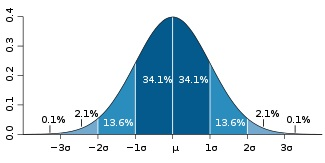
\includegraphics[height=2.5in,width=3.2in]{chapter4/normaldistribution.jpg}
\end{center}



\textbf{Properties of the $N(\mu,\sigma^2)$ RV}
\bi
\item  \underbar{~~~~~~~~~~~~~~~~~~~~~~~~~~~~~~~~~~~~~~~~~~~~~~~~~~~~~~~~~~~~~~~~~~~~~~~~~~~~~~~~~~~~~~~} \\
\item  \underbar{~~~~~~~~~~~~~~~~~~~~~~~~~~~~~~~~~~~~~~~~~~~~~~~~~~~~~~~~~~~~~~~~~~~~~~~~~~~~~~~~~~~~~~~} \\
\item  \underbar{~~~~~~~~~~~~~~~~~~~~~~~~~~~~~~~~~~~~~~~~~~~~~~~~~~~~~~~~~~~~~~~~~~~~~~~~~~~~~~~~~~~~~~~} 
\ei
\textbf{Expectation and Variance of $N(\mu,\sigma^2)$.}:\\
$$E(Y) = \underbar{~~~~~~~~~~~~~~~~} , ~~~ Var(Y) = \underbar{~~~~~~~~~~~~~~~~~~~} .$$
Note: these are the parameters of the distribution - (i.e. the distribution is  \underbar{~~~~~~~~~~~~~~~~~~~~~~~~~~~~~~~~~~~~~}  by its mean and variance)

\pagebreak

$Z\sim N(0,1)$ (i.e. a normal distribution with $\mu=0$ and $\sigma^2=1$) is said to follow a \\~\\~\\
The standard normal is centered at zero and its probabilities are concentrated between (-3,+3).
\begin{center}
\vspace{-10pt}
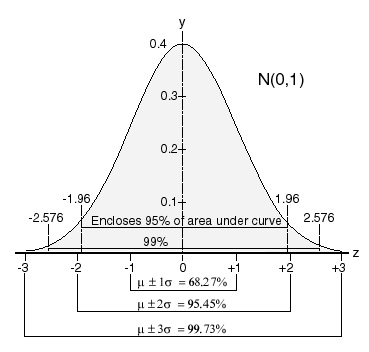
\includegraphics[height=2.5in,width=3in]{chapter4/stdnormaldistribution.jpg}
\end{center}


\textbf{Standardization of Normal Random Variables Theorem}\\~\\~\\
If $Y \sim N(\mu, \sigma^2)$, then  \underbar{~~~~~~~~~~~~~~~~~~~~~~~~~~~~~~~~~~~~~~~~~~~~~}  follows the std normal distribution:\\~\\~\\~\\~\\
Suppose that $Y \sim N(\mu, \sigma^2)$. By standardizing $Y$, we have\\~\\~\\~\\~\\~\\~\\
Likewise,  if $Z\sim N(0,1)$ \underbar{~~~~~~~~~~~~~~~~~~~~~~~~~~~~~~~~~~~~~~~~~~~~~~~~~~~~~~~} \\~\\

\textbf{CDF of $Z \sim N(0, 1)$: $\Phi(z)$}\\
The CDF (cumulative distribution function) of the standard normal random variable $Z$ is by definition:\\~\\~\\~\\~\\~\\
No closed form, has to be calculated through  \underbar{~~~~~~~~~~~~~~~~~~~~~~~~~~~~~~~~~~~~~~~~~~~~~~~~~~~~} .\\~\\
Tables or calculators often used.

\pagebreak

We will use SAS to find probabilities (for homework, on test you will just need to find the answer in terms of a standard normal distribution).  See SAS file on web.\\~\\

\textbf{Bottle Example}\\
A company that manufactures and bottles apple juice uses a machine that automatically fills 16-ounce bottles.  There is some variation, however, in the amounts of liquid dispensed into the bottles.  The amount dispensed has been observed to be approximately normally distributed with mean 16 ounces and standard deviation 1 ounce. \\
What is the probability a randomly selected bottle will:
\bi
\item have more than 17.5 ounces?\\~\\~\\~\\~\\~\\~\\~\\~\\
\item have between 15.2 and 16 ounces?\\~\\~\\~\\~\\~\\~\\~\\~\\
\item have less than 15 ounces?\\~\\~\\~\\~\\~\\~\\~\\~\\~\\~\\~\\~\\~\\~\\~\\~\\
(See example 4.15, 4.16, 4.17 in the book on page 174 for more practice.)
\ei

\pagebreak

\textbf{Percentiles of the Normal Distribution}\\
The \textbf{$(100p)$th percentile} of $Y$ (also called the \textbf{pth quantile} of $Y$) is the value y that solves $P(Y \leq y) = p$. \\~\\
Suppose $Z \sim N(0,1)$. Find (see SAS file)
\be
\item the 97.5th percentile of $Z$: $z=$\\~\\~\\~\\~\\~\\~\\~\\~\\
\item the 2.5th percentile of $Z$: $z=$\\~\\~\\~\\~\\~\\~\\~\\~\\
\ee
Suppose $Y \sim N(100, 9)$. Then find
\be
\item the 97.5th percentile of $Y$: $y=$\\~\\~\\~\\~\\~\\~\\~\\~\\
\item the 2.5th percentile of $Y$: $y=$\\~\\~\\~\\~\\~\\~\\~\\~\\~\\
\ee
(See examples 4.18 and 4.19 on page 177/178 for more practice.)
\pagebreak

\textbf{SAT/ACT Example}\\
The mathematics portion of the SAT and ACT exams produce scores that are approximately normally distributed.  The SAT scores have averaged 480 with a S.D. of 100.  The ACT scores average 18 with a S.D. of 6.
\be
\item An engineering school sets 550 as the minimum SAT math score for students.  What percentage of students will score below 550 typically?\\~\\~\\~\\~\\~\\~\\~\\~\\~\\~\\~\\~\\~\\~\\~\\
\item What score should the engineering school set as a comparable standard on the ACT?
\ee









